\documentclass{article}
\usepackage{tikz}
\usetikzlibrary{patterns,decorations.pathmorphing,positioning, shapes.multipart, calc,arrows, shapes.geometric}
\usepackage[dvipsnames]{xcolor}

\begin{document}
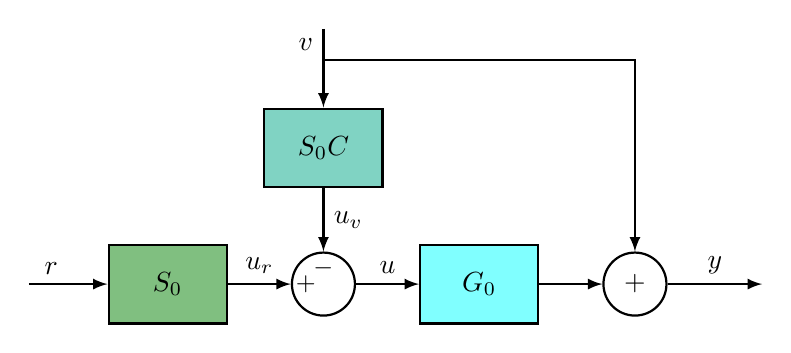
\begin{tikzpicture}[circ/.style = {draw, circle, minimum size=8mm, inner sep=0pt}, thick ]

% S0 -  Referential Origin
\node[draw, fill=Green!50, minimum width=15mm, minimum height=10mm ] (S0) at (0,0){$S_0$};

% sum_u
\node[circ , right=8mm of S0 ]  (sum_u) {};
\node[left=-1pt] at (sum_u.center){\small $+$};
\node[above=-1pt] at (sum_u.center){\small $-$};

% G0
\node[draw, fill=Cyan!50, minimum width=15mm, minimum height=10mm , right=8mm of sum_u ] (G0)    {$G_0$};

% sum_v
\node[circ, , right=8mm of G0 ]  (sum_v) {$+$};

% S0C
\node[draw, fill=Emerald!50, minimum width=15mm, minimum height=10mm, above=8mm of sum_u ] (S0C)  {$S_{0}C$};

% %--- Input r2 ---
% \draw[-latex] (-1.5, 0) -- node[above]{$r_2$} (sum_r2);

%--- r -> S0
\draw[-latex] ([xshift=-10mm]S0.west) -- node[left, yshift=2mm]{$r$} (S0);

%--- S0 -> u_r
\draw[-latex] (S0) -- node[above] {$u_r$} (sum_u);
% %--- r1 drops into sum_u from above ---
% \draw[-latex] ([yshift=10mm]sum_u.north) node[left ,yshift=-2mm]{$r_1$} -- (sum_u);

%--- sum_u -> G0 ---
\draw[-latex] (sum_u) -- node[above]{$u$} (G0);

%--- G0 -> sum_v ---
\draw[-latex] (G0) -- (sum_v);

%--- v -> S0C -> u_v -> sum_v ---
\draw[-latex] ([yshift=10mm]S0C.north) node[left,yshift=-2mm]{$v$} -- (S0C);
\draw[-latex] (S0C) -- node[right]{$u_v$} (sum_u);

%--- sum_v -> y output ---
\draw[-latex] (sum_v) -- node[above]{$y$} ([xshift=12mm] sum_v.east);

%--- v branches to sum_v
\coordinate (ybranch) at ([yshift=6mm] S0C.north);
\draw [-latex] (ybranch) -- (ybranch -| sum_v) -- (sum_v.north);

% % grid for debug   %% this i what you get for hardcoding the coordinates which should be relative
% \draw[gray!40, step=0.5] (-1,-3) grid (12,3); 
% \draw[gray,    step=1]   (-1,-3) grid (12,3);
% \foreach \x in {-1,0,...,12} \node[below, gray, font=\tiny] at (\x,-3) {\x};
% \foreach \y in {-3,-2,...,3}  \node[left,  gray, font=\tiny] at (-1,\y) {\y};

\end{tikzpicture}
\end{document}
